%To compile as handout, use
%pdflatex "\def\ishandout{1} \input{filename.tex}"
%Defaults to non-handout mode (with slide reveals)
\ifdefined\ishandout
  \documentclass[handout]{beamer}
\else
  \documentclass{beamer}
\fi
 
\usepackage{econ103slides} 

\date{Lecture \# 10}
\begin{document} 

%%%%%%%%%%%%%%%%%%%%%%%%%%%%%%%%%%%%%%%%

\begin{frame}[plain]
	\titlepage 
	

\end{frame} 

%%%%%%%%%%%%%%%%%%%%%%%%%%%%%%%%%%%%%%%%
\begin{frame}

\centering \Huge Discrete RVs -- Part III

\end{frame}
%%%%%%%%%%%%%%%%%%%%%%%%%%%%%%%%%%%%%%%%
\begin{frame}
\frametitle{Overview}

\begin{block}{So Far}
Consider one RV at a time.
\end{block}

\begin{block}{Today}
Consider relationships \emph{between} RVs.
\end{block}

\end{frame}
%%%%%%%%%%%%%%%%%%%%%%%%%%%%%%%%%%%%%%%%
\begin{frame}
\frametitle{Definition of Joint PMF}
Let $X$ and $Y$ be discrete random variables. The joint probability mass function $p_{XY}(x,y)$ gives the probability of each pair of realizations $(x,y)$ in the support:
\Large
 $$\boxed{p_{XY}(x,y) = P(X = x \cap Y=y)}$$

\end{frame}
%%%%%%%%%%%%%%%%%%%%%%%%%%%%%%%%%%%%%%%%
\begin{frame}
\frametitle{Example: Joint PMF in Tabular Form}

\begin{table}
\begin{tabular}{|cc|ccc|}
\hline
&&\multicolumn{3}{c|}{$Y$}\\
&&1 & 2&3\\
\hline
\multirow{4}{*}{$X$}
&0& \multicolumn{1}{|c}{\alert{1/8}} & \alert{0}& \alert{0}\\
&1& \multicolumn{1}{|c}{\alert{0}} & \alert{1/4}&\alert{1/8}\\
&2& \multicolumn{1}{|c}{\alert{0}} & \alert{1/4}&\alert{1/8}\\
&3& \multicolumn{1}{|c}{\alert{1/8}} & \alert{0}&\alert{0}\\
\hline
\end{tabular}
\end{table}

\end{frame}
%%%%%%%%%%%%%%%%%%%%%%%%%%%%%%%%%%%%%%%%
\begin{frame}
\frametitle{Plot of Joint PMF}
\begin{figure}
	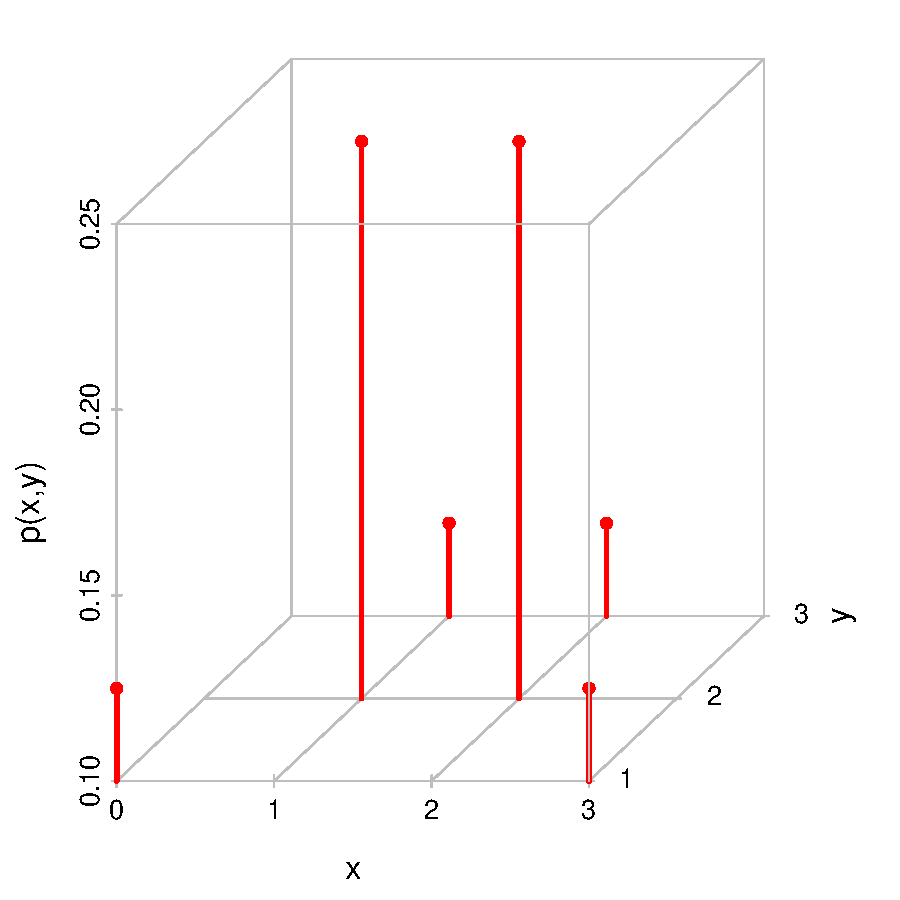
\includegraphics[scale = 0.53]{./images/joint_dist}
\end{figure}

\end{frame}



%%%%%%%%%%%%%%%%%%%%%%%%%%%%%%%%%%%%%%%%
\begin{frame}
\frametitle{What is $p_{XY}(1,2)$? \hfill 
\includegraphics[scale = 0.05]{./images/clicker}}

\begin{table}
\begin{tabular}{|cc|ccc|}
\hline
&&\multicolumn{3}{c|}{$Y$}\\
&&1 & 2&3\\
\hline
\multirow{4}{*}{$X$}
&0& \multicolumn{1}{|c}{\alert{1/8}} & \alert{0}& \alert{0}\\
&1& \multicolumn{1}{|c}{\alert{0}} & \alert{1/4}&\alert{1/8}\\
&2& \multicolumn{1}{|c}{\alert{0}} & \alert{1/4}&\alert{1/8}\\
&3& \multicolumn{1}{|c}{\alert{1/8}} & \alert{0}&\alert{0}\\
\hline
\end{tabular}
\end{table}

\pause



$$p_{XY}(1,2) =   P(X=1 \cap Y =2) =  \alert{1/4}$$

\end{frame}

%%%%%%%%%%%%%%%%%%%%%%%%%%%%%%%%%%%%%%%%
\begin{frame}
\frametitle{What is $p_{XY}(2,1)$? \hfill 
\includegraphics[scale = 0.05]{./images/clicker}}

\begin{table}
\begin{tabular}{|cc|ccc|}
\hline
&&\multicolumn{3}{c|}{$Y$}\\
&&1 & 2&3\\
\hline
\multirow{4}{*}{$X$}
&0& \multicolumn{1}{|c}{\alert{1/8}} & \alert{0}& \alert{0}\\
&1& \multicolumn{1}{|c}{\alert{0}} & \alert{1/4}&\alert{1/8}\\
&2& \multicolumn{1}{|c}{\alert{0}} & \alert{1/4}&\alert{1/8}\\
&3& \multicolumn{1}{|c}{\alert{1/8}} & \alert{0}&\alert{0}\\
\hline
\end{tabular}
\end{table}

\pause

$$p_{XY}(2,1) =  P(X=2 \cap Y =1) = \alert{0}$$

\end{frame}

%%%%%%%%%%%%%%%%%%%%%%%%%%%%%%%%%%%%%%%%

\begin{frame}
\frametitle{Properties of Joint PMF}
	\begin{enumerate}
		\item $0\leq p_{XY}(x,y)\leq 1$ for any pair $(x,y)$
		\item The sum of $p_{XY}(x,y)$ over all pairs $(x,y)$ in the support is 1:
			$$\sum_{x}\sum_{y} p(x,y) = 1$$
	\end{enumerate}
\end{frame}


%%%%%%%%%%%%%%%%%%%%%%%%%%%%%%%%%%%%%%%%
\begin{frame}
\frametitle{Does this satisfy the properties of a joint pmf? \hfill 
\includegraphics[scale = 0.05]{./images/clicker}}
\alert{(A = YES, B = NO)}
\begin{table}
\begin{tabular}{|cc|ccc|}
\hline
&&\multicolumn{3}{c|}{$Y$}\\
&&1 & 2&3\\
\hline
\multirow{4}{*}{$X$}
&0& \multicolumn{1}{|c}{\alert{1/8}} & \alert{0}& \alert{0}\\
&1& \multicolumn{1}{|c}{\alert{0}} & \alert{1/4}&\alert{1/8}\\
&2& \multicolumn{1}{|c}{\alert{0}} & \alert{1/4}&\alert{1/8}\\
&3& \multicolumn{1}{|c}{\alert{1/8}} & \alert{0}&\alert{0}\\
\hline
\end{tabular}
\end{table}

\pause

\begin{enumerate}
	\item $p(x,y) \geq 0$ for all pairs $(x,y)$
	\item $\sum_x\sum_{y} p(x,y) = 1/8 + 1/4 + 1/8 + 1/4 + 1/8 + 1/8 = 1$
\end{enumerate}

\end{frame}

%%%%%%%%%%%%%%%%%%%%%%%%%%%%%%%%%%%%%%%%
\begin{frame}
\frametitle{Joint versus Marginal PMFs}

\begin{block}{Joint PMF}
 $p_{XY}(x,y) = P(X=x \cap Y=y)$
\end{block}



\begin{block}{Marginal PMFs}
$p_X(x) = P(X=x)$\\ $p_Y(y) = P(Y=y)$
\end{block}



\vspace{1em}

\alert{You can't calculate a joint pmf from marginals alone but you \emph{can} calculate marginals from the joint!}

\end{frame}
%%%%%%%%%%%%%%%%%%%%%%%%%%%%%%%%%%%%%%%%
\begin{frame}
\frametitle{Marginals from Joint}

	$$\boxed{p_X(x) = \sum_{\mbox{all } y} p_{XY}(x,y)}$$
	
	$$\boxed{p_Y(y) = \sum_{\mbox{all } x} p_{XY}(x,y)}$$


\begin{block}{Why?}
	\begin{eqnarray*}
	p_Y(y) &=& P(Y=y) = P\left( \bigcup_{\mbox{all } x}\left\{ X=x \cap Y=y \right\}  \right)\\
		&=& \sum_{\mbox{all } x} P(X=x \cap Y=y) = \sum_{\mbox{all } x} p_{XY}(x,y)
	\end{eqnarray*}
\end{block}
\end{frame}
%%%%%%%%%%%%%%%%%%%%%%%%%%%%%%%%%%%%%%%%
\begin{frame}
\frametitle{To get the marginals sum ``into the margins'' of the table.}

\begin{table}
\begin{tabular}{|cc|ccc|c|}
\hline
&&\multicolumn{3}{c|}{$Y$}&\\
&&1 & 2&3&\\
\hline
\multirow{4}{*}{$X$}
&0& \multicolumn{1}{|c}{\alert{1/8}} & \alert{0}& \alert{0}&\onslide<2->{\textcolor{blue}{1/8}}\\
&1& \multicolumn{1}{|c}{\alert{0}} & \alert{1/4}&\alert{1/8}&\onslide<3->{\textcolor{blue}{3/8}}\\
&2& \multicolumn{1}{|c}{\alert{0}} & \alert{1/4}&\alert{1/8}&\onslide<4->{\textcolor{blue}{3/8}}\\
&3& \multicolumn{1}{|c}{\alert{1/8}} & \alert{0}&\alert{0}&\onslide<5->{\textcolor{blue}{1/8}}\\
\hline 
&&&&&\onslide<5->{\textcolor{blue}{1}}\\
\hline
\end{tabular}
\end{table}

\begin{eqnarray*}
	\onslide<2->{p_X(0) &=& 1/8 + 0 + 0 = 1/8}\\
	\onslide<3->{p_X(1) &=&0 + 1/4 + 1/8 = 3/8}\\
	\onslide<4->{p_X(2) &=&0 + 1/4 + 1/8 = 3/8}\\
	\onslide<5->{p_X(3) &=&1/8 + 0 + 0 = 1/8}
\end{eqnarray*}


\end{frame}

%%%%%%%%%%%%%%%%%%%%%%%%%%%%%%%%%%%%%%%%

\begin{frame}
\frametitle{What is $p_Y(2)$? \hfill 
\includegraphics[scale = 0.05]{./images/clicker}}

\begin{table}
\begin{tabular}{|cc|ccc|c|}
\hline
&&\multicolumn{3}{c|}{$Y$}&\\
&&1 & 2&3&\\
\hline
\multirow{4}{*}{$X$}
&0& \multicolumn{1}{|c}{\alert{1/8}} & \alert{0}& \alert{0}&\\
&1& \multicolumn{1}{|c}{\alert{0}} & \alert{1/4}&\alert{1/8}&\\
&2& \multicolumn{1}{|c}{\alert{0}} & \alert{1/4}&\alert{1/8}&\\
&3& \multicolumn{1}{|c}{\alert{1/8}} & \alert{0}&\alert{0}&\\
\hline 
&&\onslide<2->{\textcolor{blue}{1/4}}&\onslide<3->{ \textcolor{blue}{1/2} }& \onslide<4->{\textcolor{blue}{1/4}} &\onslide<4->{\textcolor{blue}{1}}\\
\hline
\end{tabular}
\end{table}

\begin{eqnarray*}
	\onslide<2->{p_Y(1) &=& 1/8 + 0 + 0 + 1/8 = 1/4}\\
	\onslide<3->{p_Y(2) &=&0 + 1/4 + 1/4 + 0 = 1/2}\\
	\onslide<4->{p_Y(3) &=&0 + 1/8 + 1/8 + 0= 1/4}
\end{eqnarray*}


\end{frame}

%%%%%%%%%%%%%%%%%%%%%%%%%%%%%%%%%%%%%%%%

\begin{frame}
\frametitle{Definition of Conditional PMF}
\framesubtitle{How does the distribution of $y$ change with $x$?}

\Large
$$\boxed{p_{Y|X}(y|x) = P(Y=y|X=x)}$$


\end{frame}
%%%%%%%%%%%%%%%%%%%%%%%%%%%%%%%%%%%%%%%%
\begin{frame}
\frametitle{Which of these is the formula for $p_{Y|X}(y|x)$? \hfill 
\includegraphics[scale = 0.05]{./images/clicker}}
You can figure this out from what you already know about probability, using the definition $p_{Y|X}(y|x) = P(Y=y|X=x)$

\vspace{1em}

\begin{enumerate}[(a)]
\item $p_X(x)/p_Y(y)$
\item $p_{XY}(x,y)/p_X(x)$
\item $p_X(x)p_{XY}(x,y)$
\item $p_{XY}(x,y)/p_Y(y)$
\item $p_Y(y)/p_X(x)$
\end{enumerate}

\end{frame}
%%%%%%%%%%%%%%%%%%%%%%%%%%%%%%%%%%%%%%%%
\begin{frame}
\frametitle{Conditional PMF from Joint and Marginal}

\begin{eqnarray*}
	p_{Y|X}(y|x) = P(Y=y|X=x) =  \frac{P(Y=y \cap X=x)}{P(X=x)} =  \frac{p_{XY}(x,y)}{p_X(x)}
\end{eqnarray*}
\vspace{1em}

Hence,
 $$\boxed{p_{Y|X}(y|x) = \frac{p_{XY}(x,y)}{p_X(x)}}$$
 and similarly,
  $$\boxed{p_{X|Y}(x|y) = \frac{p_{XY}(x,y)}{p_Y(y)}}$$

\end{frame}


%%%%%%%%%%%%%%%%%%%%%%%%%%%%%%%%%%%%%%%%
\begin{frame}
\frametitle{Conditional PMF of $Y$ given $X = 2$}

\begin{table}
\begin{tabular}{|cc|ccc|c|}
\hline
&&\multicolumn{3}{c|}{$Y$}&\\
&&1 & 2&3&\\
\hline
\multirow{4}{*}{$X$}
&0& \multicolumn{1}{|c}{1/8} & 0& 0&1/8\\
&1& \multicolumn{1}{|c}{0} & 1/4&1/8&3/8\\
&2& \multicolumn{1}{|c}{\alert{0}} & \alert{1/4}&\alert{1/8}&\textcolor{blue}{3/8}\\
&3& \multicolumn{1}{|c}{1/8} & 0&0&1/8\\
\hline
\end{tabular}
\end{table}

\begin{eqnarray*}
	p_{Y|X}(1|2) &=&\pause \frac{p_{XY}(2,1)}{p_X(2)} =\pause \frac{0}{3/8} =\alert{0}\\ \\ \pause
	p_{Y|X}(2|2) &=&\frac{p_{XY}(2,2)}{p_X(2)}= \frac{1/4}{3/8} =\alert{2/3} \\ \\ \pause
	 p_{Y|X}(3|2) &=&\frac{p_{XY}(2,3)}{p_X(2)} = \frac{1/8}{3/8} = \alert{1/3}
\end{eqnarray*}


\end{frame}
%%%%%%%%%%%%%%%%%%%%%%%%%%%%%%%%%%%%%%%%
\begin{frame}
\frametitle{What is $p_{X|Y}(1|2)$? \hfill 
\includegraphics[scale = 0.05]{./images/clicker}}
\small
\begin{table}
\begin{tabular}{|cc|ccc|c|}
\hline
&&\multicolumn{3}{c|}{$Y$}&\\
&&1 & 2&3&\\
\hline
\multirow{4}{*}{$X$}
&0& \multicolumn{1}{|c}{1/8} & \alert{0}&0&\\
&1& \multicolumn{1}{|c}{0} & \alert{1/4}&1/8&\\
&2& \multicolumn{1}{|c}{0} & \alert{1/4}&1/8&\\
&3& \multicolumn{1}{|c}{1/8} & \alert{0}&0&\\
\hline 
&&1/4&\textcolor{blue}{1/2}&1/4&\\
\hline
\end{tabular}
\end{table}

\pause
\begin{eqnarray*}
	p_{X|Y}(0|2) &=&\frac{p_{XY}(0,2)}{p_Y(2)} = \frac{0}{1/2} = 0\\ \pause
	p_{X|Y}(1|2) &=&\frac{p_{XY}(1,2)}{p_Y(2)}=\frac{1/4}{1/2}= \alert{1/2}\\ \pause
	 p_{X|Y}(2|2) &=&\frac{p_{XY}(2,2)}{p_Y(2)}=\frac{1/4}{1/2}= 1/2\\ \pause
	 	 p_{X|Y}(3|2) &=&\frac{p_{XY}(3,2)}{p_Y(2)}=\frac{0}{1/2} = 0\\
\end{eqnarray*}


\end{frame}

%%%%%%%%%%%%%%%%%%%%%%%%%%%%%%%%%%%%%%%%


\begin{frame}
\frametitle{Independent RVs}


\begin{block}{Definition}
We say that two discrete RVs are \alert{independent} if and only if their joint pmf equals the product of their marginal pmfs: $$p_{XY}(x,y) = p_X(x)p_Y(y)$$ for all pairs $(x,y)$ in the support.
\end{block}


\begin{block}{In Terms of Conditional PMF}
From the previous slide, it follows that an equivalent definition of independence is that both conditional pmfs equal the corresponding marginal pmfs: $p_{Y|X}(y|X) = p_Y(y)$ and  $p_{X|Y}(x|y) = p_X(x)$ for all $(x,y)$ in the support.
\end{block}

\end{frame}
%%%%%%%%%%%%%%%%%%%%%%%%%%%%%%%%%%%%%%%%
\begin{frame}
\frametitle{Are $X$ and $Y$ Independent? \hfill 
\includegraphics[scale = 0.05]{./images/clicker}}
\alert{(A = YES, B = NO)}
\small
\begin{table}
\begin{tabular}{|cc|ccc|c|}
\hline
&&\multicolumn{3}{c|}{$Y$}&\\
&&1 & 2&3&\\
\hline
\multirow{4}{*}{$X$}
&0& \multicolumn{1}{|c}{\alert{1/8}} & \alert{0}& \alert{0}&\textcolor{blue}{1/8}\\
&1& \multicolumn{1}{|c}{\alert{0}} & \alert{1/4}&\alert{1/8}&\textcolor{blue}{3/8}\\
&2& \multicolumn{1}{|c}{\alert{0}} & \alert{1/4}&\alert{1/8}&\textcolor{blue}{3/8}\\
&3& \multicolumn{1}{|c}{\alert{1/8}} & \alert{0}&\alert{0}&\textcolor{blue}{1/8}\\
\hline
&&\textcolor{blue}{1/4}&\textcolor{blue}{1/2}&\textcolor{blue}{1/4}&\\
\hline
\end{tabular}
\end{table}

\pause

\begin{eqnarray*}
	p_{XY}(2,1) &=& 0\\ \pause
	p_X(2) \times p_Y(1) &=& \pause (3/8) \times (1/4) \neq 0
\end{eqnarray*}

\alert{Therefore $X$ and $Y$ are \emph{not} independent.}
\end{frame}
%%%%%%%%%%%%%%%%%%%%%%%%%%%%%%%%%%%%%%%%
\begin{frame}
\frametitle{Conditional Expectation}
\begin{block}{Intuition}
	$E[Y|X]$ is our ``best guess'' of the realization that $Y$ will take on having observed the realization of $X$.
\end{block}
\pause

\begin{block}{$E[Y|X]$ is a Random Variable}
Unlike $E[Y]$ which is a constant, $E[Y|X]$ is a function of $X$, hence it is a \alert{Random Variable}.
\end{block}
\pause

\begin{block}{$E[Y|X=x]$ is a Constant}
To get a ``best guess'' for $Y$, we plug in the realization we observed for $X$: $E[Y|X=x]$ is a constant, our guess of the realization of $Y$.
\end{block}\pause

\begin{block}{Calculating $E[Y|X=x]$}
Take the mean of the conditional pmf of $Y$ given $X=x$.
\end{block}

\end{frame}
%%%%%%%%%%%%%%%%%%%%%%%%%%%%%%%%%%%%%%%%
\begin{frame}
	\frametitle{Conditional Expectation: $E[Y|X=2]$}

\footnotesize
\begin{table}
\begin{tabular}{|cc|ccc|c|}
\hline
&&\multicolumn{3}{c|}{$Y$}&\\
&&1 & 2&3&\\
\hline
\multirow{4}{*}{$X$}
&0& \multicolumn{1}{|c}{\alert{1/8}} & \alert{0}& \alert{0}&\textcolor{blue}{1/8}\\
&1& \multicolumn{1}{|c}{\alert{0}} & \alert{1/4}&\alert{1/8}&\textcolor{blue}{3/8}\\
&2& \multicolumn{1}{|c}{\alert{0}} & \alert{1/4}&\alert{1/8}&\textcolor{blue}{3/8}\\
&3& \multicolumn{1}{|c}{\alert{1/8}} & \alert{0}&\alert{0}&\textcolor{blue}{1/8}\\
\hline
&&\textcolor{blue}{1/4}&\textcolor{blue}{1/2}&\textcolor{blue}{1/4}&\\
\hline
\end{tabular}
\end{table}

We showed above that the conditional pmf of $Y|X=2$ is:
	$$\boxed{\begin{array}{ccc}p_{Y|X}(1|2) =0 \quad&p_{Y|X}(2|2) =2/3 \quad&p_{Y|X}(3|2) =1/3\end{array}}$$
	
	
Hence
	$$E[Y|X=2] = 2 \times 2/3 + 3 \times 1/3 =  \alert{7/3}$$

\end{frame}
%%%%%%%%%%%%%%%%%%%%%%%%%%%%%%%%%%%%%%%%
\begin{frame}
	\frametitle{Conditional Expectation: $E[Y|X=0]$}

\footnotesize
\begin{table}
\begin{tabular}{|cc|ccc|c|}
\hline
&&\multicolumn{3}{c|}{$Y$}&\\
&&1 & 2&3&\\
\hline
\multirow{4}{*}{$X$}
&0& \multicolumn{1}{|c}{\alert{1/8}} & \alert{0}& \alert{0}&\textcolor{blue}{1/8}\\
&1& \multicolumn{1}{|c}{\alert{0}} & \alert{1/4}&\alert{1/8}&\textcolor{blue}{3/8}\\
&2& \multicolumn{1}{|c}{\alert{0}} & \alert{1/4}&\alert{1/8}&\textcolor{blue}{3/8}\\
&3& \multicolumn{1}{|c}{\alert{1/8}} & \alert{0}&\alert{0}&\textcolor{blue}{1/8}\\
\hline
&&\textcolor{blue}{1/4}&\textcolor{blue}{1/2}&\textcolor{blue}{1/4}&\\
\hline
\end{tabular}
\end{table}

The conditional pmf of $Y|X=0$ is 
	$$\boxed{\begin{array}{ccc}p_{Y|X}(1|0) =1 \quad&p_{Y|X}(2|0) =0 \quad&p_{Y|X}(3|0) =0\end{array}}$$
	

\alert{Hence $E[Y|X=0] = 1$}

\end{frame}
%%%%%%%%%%%%%%%%%%%%%%%%%%%%%%%%%%%%%%%%
\begin{frame}
	\frametitle{Calculate $E[Y|X=3]$}

\footnotesize
\begin{table}
\begin{tabular}{|cc|ccc|c|}
\hline
&&\multicolumn{3}{c|}{$Y$}&\\
&&1 & 2&3&\\
\hline
\multirow{4}{*}{$X$}
&0& \multicolumn{1}{|c}{\alert{1/8}} & \alert{0}& \alert{0}&\textcolor{blue}{1/8}\\
&1& \multicolumn{1}{|c}{\alert{0}} & \alert{1/4}&\alert{1/8}&\textcolor{blue}{3/8}\\
&2& \multicolumn{1}{|c}{\alert{0}} & \alert{1/4}&\alert{1/8}&\textcolor{blue}{3/8}\\
&3& \multicolumn{1}{|c}{\alert{1/8}} & \alert{0}&\alert{0}&\textcolor{blue}{1/8}\\
\hline
&&\textcolor{blue}{1/4}&\textcolor{blue}{1/2}&\textcolor{blue}{1/4}&\\
\hline
\end{tabular}
\end{table}


The conditional pmf of $Y|X=3$ is
	$$\boxed{\begin{array}{ccc}p_{Y|X}(1|3) =1 \quad&p_{Y|X}(2|3) =0 \quad&p_{Y|X}(3|3) =0\end{array}}$$
	
\alert{Hence $E[Y|X=3] = 1$}

\end{frame}
%%%%%%%%%%%%%%%%%%%%%%%%%%%%%%%%%%%%%%%%
\begin{frame}
	\frametitle{Calculate $E[Y|X=1]$ \hfill 
\includegraphics[scale = 0.05]{./images/clicker}}

\footnotesize
\begin{table}
\begin{tabular}{|cc|ccc|c|}
\hline
&&\multicolumn{3}{c|}{$Y$}&\\
&&1 & 2&3&\\
\hline
\multirow{4}{*}{$X$}
&0& \multicolumn{1}{|c}{\alert{1/8}} & \alert{0}& \alert{0}&\textcolor{blue}{1/8}\\
&1& \multicolumn{1}{|c}{\alert{0}} & \alert{1/4}&\alert{1/8}&\textcolor{blue}{3/8}\\
&2& \multicolumn{1}{|c}{\alert{0}} & \alert{1/4}&\alert{1/8}&\textcolor{blue}{3/8}\\
&3& \multicolumn{1}{|c}{\alert{1/8}} & \alert{0}&\alert{0}&\textcolor{blue}{1/8}\\
\hline
&&\textcolor{blue}{1/4}&\textcolor{blue}{1/2}&\textcolor{blue}{1/4}&\\
\hline
\end{tabular}
\end{table}
\pause
The conditional pmf of $Y|X=1$ is
	$$\boxed{\begin{array}{ccc}p_{Y|X}(1|1) =0 \quad&p_{Y|X}(2|1) =2/3 \quad&p_{Y|X}(3|1) =1/3\end{array}}$$
	

Hence
	$$E[Y|X=1] = 2 \times 2/3 + 3 \times 1/3 = \alert{7/3}$$

\end{frame}
%%%%%%%%%%%%%%%%%%%%%%%%%%%%%%%%%%%%%%%%
\begin{frame}
\frametitle{$E[Y|X]$ is a Random Variable}
In this particular example we have seen that:
	$$E[Y|X]= \left\{\begin{array}{cc}  
	1& X = 0\\
	7/3& X = 1\\
	7/3& X = 2\\ 
	1& X = 3 
	\end{array}\right.$$ 
But from above we know the marginal distribution of $X:$
	\begin{eqnarray*}
		P(X=0)= 1/8 && P(X=1) = 3/8\\
		P(X=2)=3/8 && P(X=3)=1/8
	\end{eqnarray*} \pause
\alert{Therefore, $E[Y|X]$ is a RV that takes on the value 1 with probability 1/4 and the value 7/3 with probability 3/4.}

\end{frame}
%%%%%%%%%%%%%%%%%%%%%%%%%%%%%%%%%%%%%%%%
\begin{frame}
\frametitle{The Law of Iterated Expectations}
Since $E[Y|X]$ is a random variable, we can ask what its expectation is. It turns out that, for any RVs $X$ and $Y$
	$$\boxed{E\left[E\left[Y|X  \right]  \right] = E[Y]}$$
and this is called the \alert{Law of Iterated Expectations}. I've posted a proof \textcolor{blue}{\href{http://fditraglia.github.io/Econ103Public/IteratedExpectationsProof.pdf}{\fbox{HERE}}} for those who want are interested.


\vspace{2em}
\hfill This will be helpful in Econ 104...
\end{frame}
%%%%%%%%%%%%%%%%%%%%%%%%%%%%%%%%%%%%%%%%
\begin{frame}[t]
\frametitle{Law of Iterated Expectations for Our Example}

\begin{columns}
\footnotesize
\column{0.5\textwidth}
\begin{block}{Marginal pmf of $Y$}
\begin{eqnarray*}
	P(Y = 1) &=& 1/4 \\
	P(Y = 2) &=& 1/2\\
	P(Y = 3) &=& 1/4
\end{eqnarray*}
\pause

\begin{eqnarray*}
	E[Y] &=& 1\times 1/4 + 2 \times 1/2 + 3 \times 1/4\\
		&=&2
\end{eqnarray*}
\end{block}

\pause
\column{0.5\textwidth}
\begin{block}{$E[Y|X]$}
	\begin{eqnarray*}
	 E[Y|X] &=& \left\{\begin{array}{cc} 1& \mbox{w/ prob. } 1/4\\ 7/3& \mbox{w/ prob. } 3/4\end{array}\right.\\\\ \pause
	 E\left[E\left[Y|X \right] \right] &=& 1 \times 1/4 + 7/3 \times 3/4\\ 
	 &=& 2
	\end{eqnarray*}
	\vspace{1em}
\end{block}

\end{columns}

\end{frame}
%%%%%%%%%%%%%%%%%%%%%%%%%%%%%%%%%%%%%%%%
\begin{frame}
\frametitle{Expectation of Function of Two Discrete RVs}
\Large
		$$\boxed{E[g(X,Y)] = \sum_x\sum_y g(x,y)p_{XY}(x,y)}$$
\end{frame}
%%%%%%%%%%%%%%%%%%%%%%%%%%%%%%%%%%%%%%%%
\begin{frame}
\frametitle{Some Extremely Important Examples}
\framesubtitle{Same For Continuous Random Variables}
Let $\mu_X = E[X], \mu_Y = E[Y]$
\vspace{2em}

\begin{block}{Covariance}
$$\sigma_{XY} = Cov(X,Y) = E[(X-\mu_X)(Y - \mu_Y)]$$
\end{block}

\begin{block}{Correlation}
$$\rho_{XY} = Corr(X,Y) = \frac{\sigma_{XY}}{\sigma_X \sigma_Y}$$
\end{block}
\vspace{3em}
\end{frame}
%%%%%%%%%%%%%%%%%%%%%%%%%%%%%%%%%%%%%%%%
\begin{frame}
\frametitle{Shortcut Formula for Covariance}

Much easier for calculating:
 $$\boxed{Cov(X,Y) = E[XY] - E[X]E[Y]}$$


\vspace{2em}
\hfill{We'll talk more about this in an upcoming lecture...}
\end{frame}
%%%%%%%%%%%%%%%%%%%%%%%%%%%%%%%%%%%%%%%%
\begin{frame}
\frametitle{Calculating $Cov(X,Y)$}

\begin{columns}

\column{0.42\textwidth}
\begin{table}
\footnotesize
\begin{tabular}{|cc|ccc|c|}
\hline
&&\multicolumn{3}{c|}{$Y$}&\\
&&1 & 2&3&\\
\hline
\multirow{4}{*}{$X$}
&0& \multicolumn{1}{|c}{\alert{1/8}} & \alert{0}& \alert{0}&\textcolor{blue}{1/8}\\
&1& \multicolumn{1}{|c}{\alert{0}} & \alert{1/4}&\alert{1/8}&\textcolor{blue}{3/8}\\
&2& \multicolumn{1}{|c}{\alert{0}} & \alert{1/4}&\alert{1/8}&\textcolor{blue}{3/8}\\
&3& \multicolumn{1}{|c}{\alert{1/8}} & \alert{0}&\alert{0}&\textcolor{blue}{1/8}\\
\hline
&&\textcolor{blue}{1/4}&\textcolor{blue}{1/2}&\textcolor{blue}{1/4}&\\
\hline
\end{tabular}
\vspace{6em}
\end{table}


\column{0.65\textwidth}
\footnotesize
\begin{eqnarray*}
	E[X] &=&3/8 + 2 \times 3/8 + 3 \times 1/8 = 3/2\\\\ 
	E[Y] &=&1/4 + 2 \times 1/2 + 3 \times 1/4 = 2 \\ \\ \pause
	E[XY] &=& 1/4\times ( 2 + 4) + 1/8 \times (3 + 6 + 3)\\ 
		&=& 3\\ \\ \pause
	Cov(X,Y) &=& E[XY] - E[X]E[Y]\\ \pause
			&=& 3 - 3/2\times 2 = 0\\\\ \pause
	Corr(X,Y) &=& Cov(X,Y)/\left[SD(X) SD(Y) \right] = 0
\end{eqnarray*}

\end{columns}

\end{frame}
%%%%%%%%%%%%%%%%%%%%%%%%%%%%%%%%%%%%%%%%
\begin{frame}
\huge
Hence, zero covariance (correlation) does \emph{not} imply independence!

\end{frame}
%%%%%%%%%%%%%%%%%%%%%%%%%%%%%%%%%%%%%%%%
\begin{frame}
\huge
However, independence \emph{does} imply zero covariance (correlation)

\end{frame}
%%%%%%%%%%%%%%%%%%%%%%%%%%%%%%%%%%%%%%%%
\begin{frame}
\frametitle{$X,Y$ Independent $\Rightarrow Cov(X,Y) = 0$}
\begin{eqnarray*}
	Cov(X,Y) &=&\pause E[(X-\mu_X)(Y-\mu_Y)]\\
	&=&\pause \sum_x \sum_y (x - \mu_X)(y- \mu_Y)p(x,y)\\
	&=&\pause  \sum_x \sum_y (x - \mu_X)(y- \mu_Y)p(x)p(y) \\
	&=& \pause \sum_x  (x - \mu_X)p(x)\left[ \sum_y (y- \mu_Y)p(y)\right] \\
	&=& \pause E[Y- \mu_Y] \sum_x  (x - \mu_X)p(x)\\
	&=& \pause E[Y- \mu_Y]E[X- \mu_X] \\
	&=& 0
\end{eqnarray*}
\end{frame}
%%%%%%%%%%%%%%%%%%%%%%%%%%%%%%%%%%%%%%%%
\end{document}
